\section{Éclairage à l'aide de la méthode de Phong}

Pour gérer l'éclairage nous utilisons la méthode de Phong~:
\begin{itemize}
    \item Composante ambiante.
    \item Composante diffuse.
    \item Composante spéculaire.
\end{itemize}

De plus différent types de lumières sont également implémentées~:
\begin{itemize}
    \item Lumière directionnelle.
    \item Lumière localisée.
    \item Spot.
\end{itemize}

{\centering
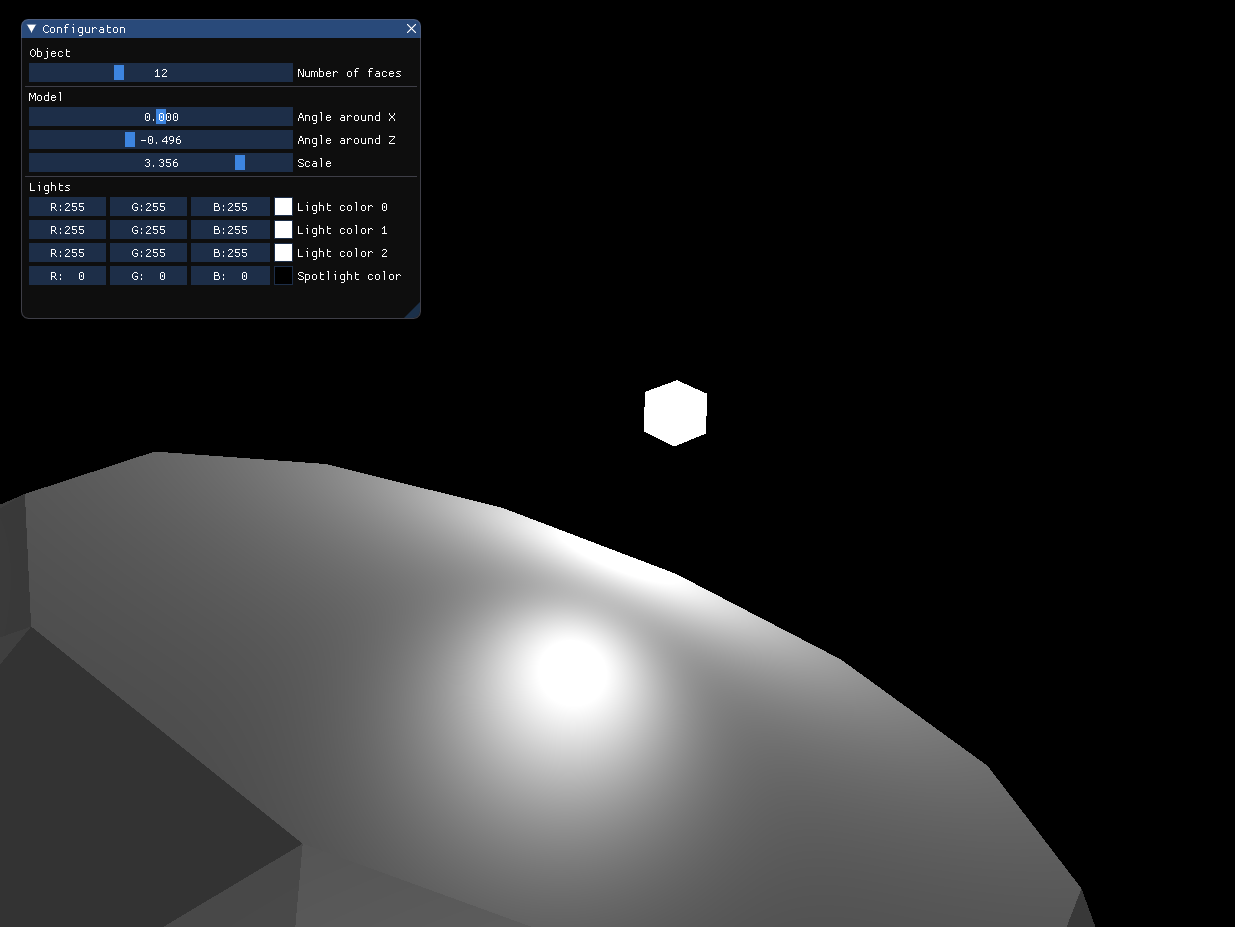
\includegraphics[width=0.9\textwidth]{screenshot_software_3}}

Notre implémentation permet de gérer un nombre arbitraire de lampes selon des constantes
définies dans le fragment shader (actuellement, aribitrairement configuré sur 5
lumières directionnelles, 15 lumières localisée et 15 spots au maximum).

